\chapter{Introduction}
In this course, we will study the principles of modeling and analysis biology
data using simulation and AI models.

In the field of biology, the scale size varies from the organism like tree passing
through tissues and arriving at the cellular level. So we are considering elements
with the size that varies from meters to micrometers.

In particular, we can distinguish two main groups of organisms: bacteria and eukaryotes.

All this organisms have in common that all have DNA as genetic material. The DNA is
a molecule that contains the information necessary to build and maintain an organism.

We can describe the DNA as a sequence of nucleotides. The nucleotides are the building
blocks of DNA. The DNA is a double helix structure, and the nucleotides are paired in
a specific way. The nucleotides are \textit{adenine}, \textit{thymine}, \textit{cytosine},
and \textit{guanine}.

This nucleotides are paired in the following way: \textit{adenine} with \textit{thymine}
and \textit{cytosine} with \textit{guanine}. This help us to save up space because
they are always complementary.

A \textbf{gene} is a sequence of nucleotides that contains the information to 
create a protein. While a \textbf{genome} is the complete set of genes of an organism.

\begin{figure}[!ht]
    \centering
    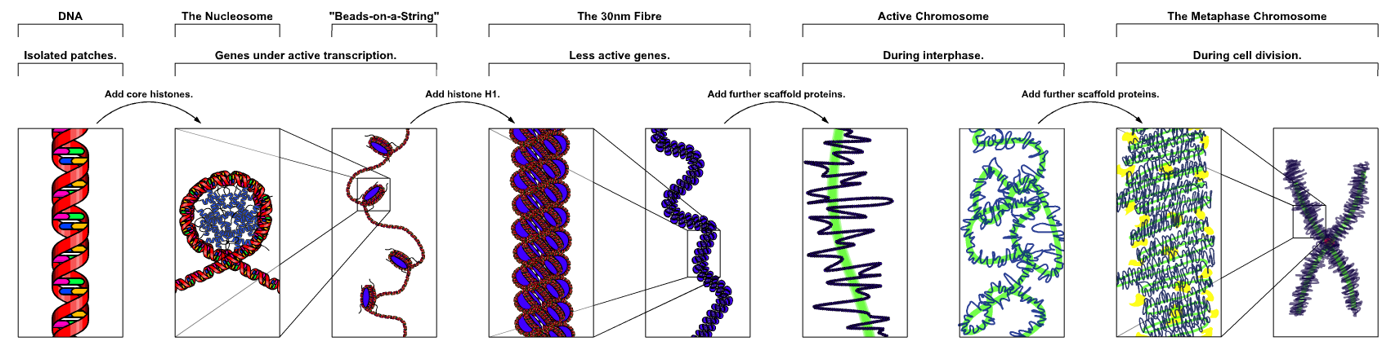
\includegraphics[width=\textwidth]{img/DNA.png}
    \caption{DNA structure}
    \label{fig:dna}
\end{figure}

A \textbf{genomic arm} refers to a large segment of a chromosome, typically 
spanning several megabases (Mb) in size.

Starting from DNA we can create \textbf{RNA} through a process called \textbf{transcription}.
The RNA is a molecule that is used to create proteins. The proteins are the building blocks
of the cells. The process of creating proteins from RNA is called \textbf{translation}.